El modelo de Schooledule se fundamenta en un modelo de capas que separa responsabilidades y garantiza el aislamiento de datos entre centros educativos.

\section{Casos de Uso Principales}
Se han identificado tres roles fundamentales en el sistema:

\begin{description}
    \item[Administrador] Gestión global de sedes, usuarios y auditoría del sistema.
    \item[Profesor] Gestión de módulos asignados, definición de ítems evaluables y calificación de alumnos.
    \item[Alumno] Consulta de progreso académico, horarios y perfil personal.
\end{description}

\begin{figure}[H]
    \centering
    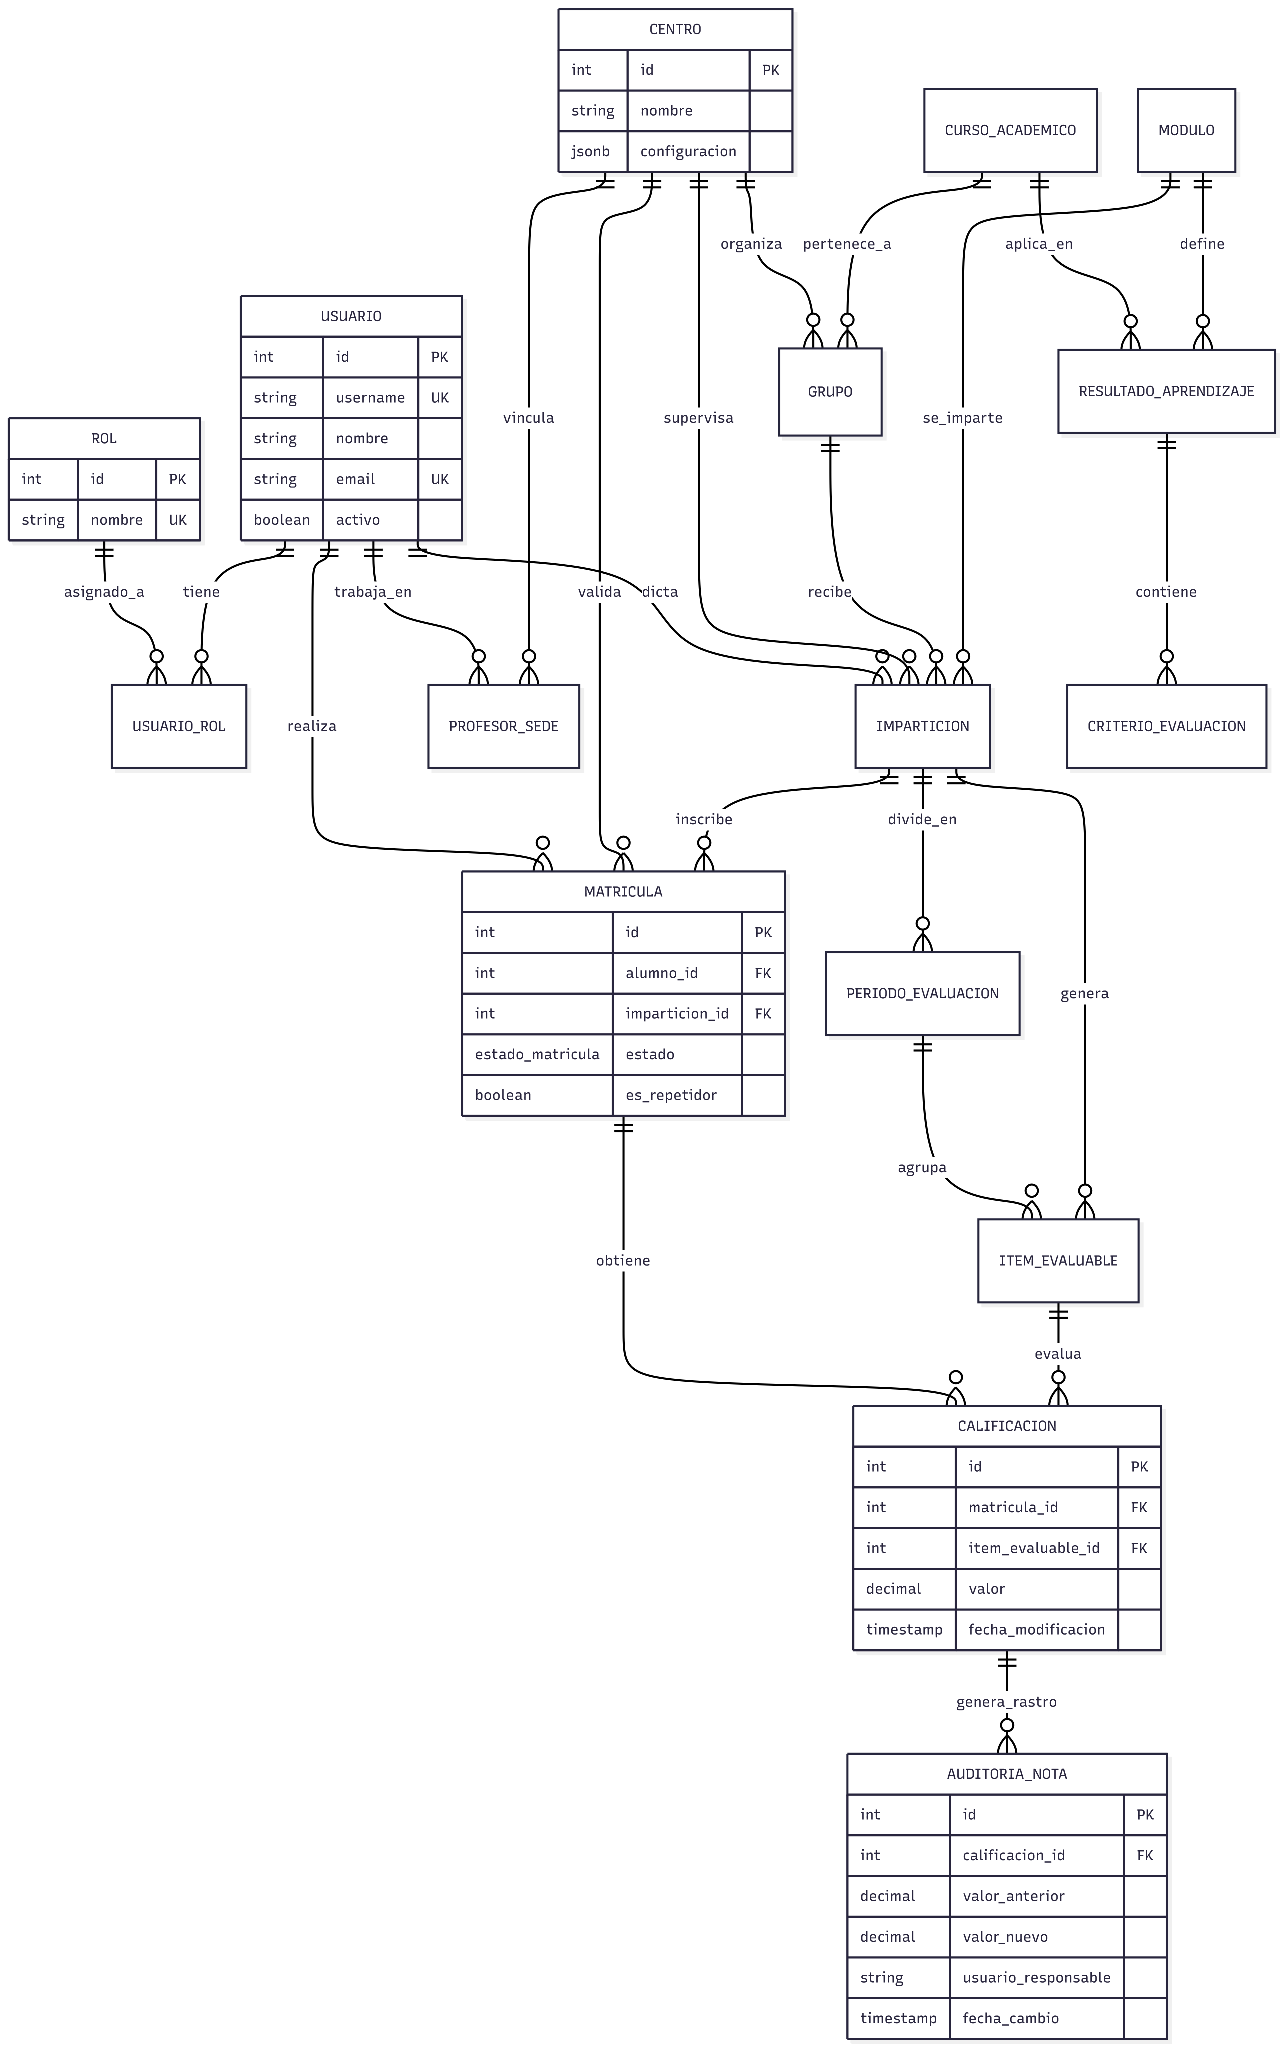
\includegraphics[width=0.9\textwidth]{figuras/image6.png}
    \caption{Diagrama de Casos de Uso del sistema Schooledule.}
    \label{fig:casos_uso}
\end{figure}

\section{Modelo de Datos y Entidades}
El diseño del modelo de dominio sigue principios de Diseño Orientado al Dominio (DDD):

\begin{description}
    \item[Centro] Representa la sede física y lógica. Eje del aislamiento multi-sede mediante el campo \texttt{centro\_id}.
    \item[Usuario y Rol] Relación N:M que permite que un usuario posea varios perfiles (ej. administrador y profesor) en una misma sede.
    \item[Impartición] Nodo central que vincula el Módulo, el Profesor, el Grupo y el Centro.
    \item[Calificación y Auditoría] Almacenamiento de notas vinculado a un registro de \texttt{AuditoriaNota} inmutable.
\end{description}

\begin{figure}[H]
    \centering
    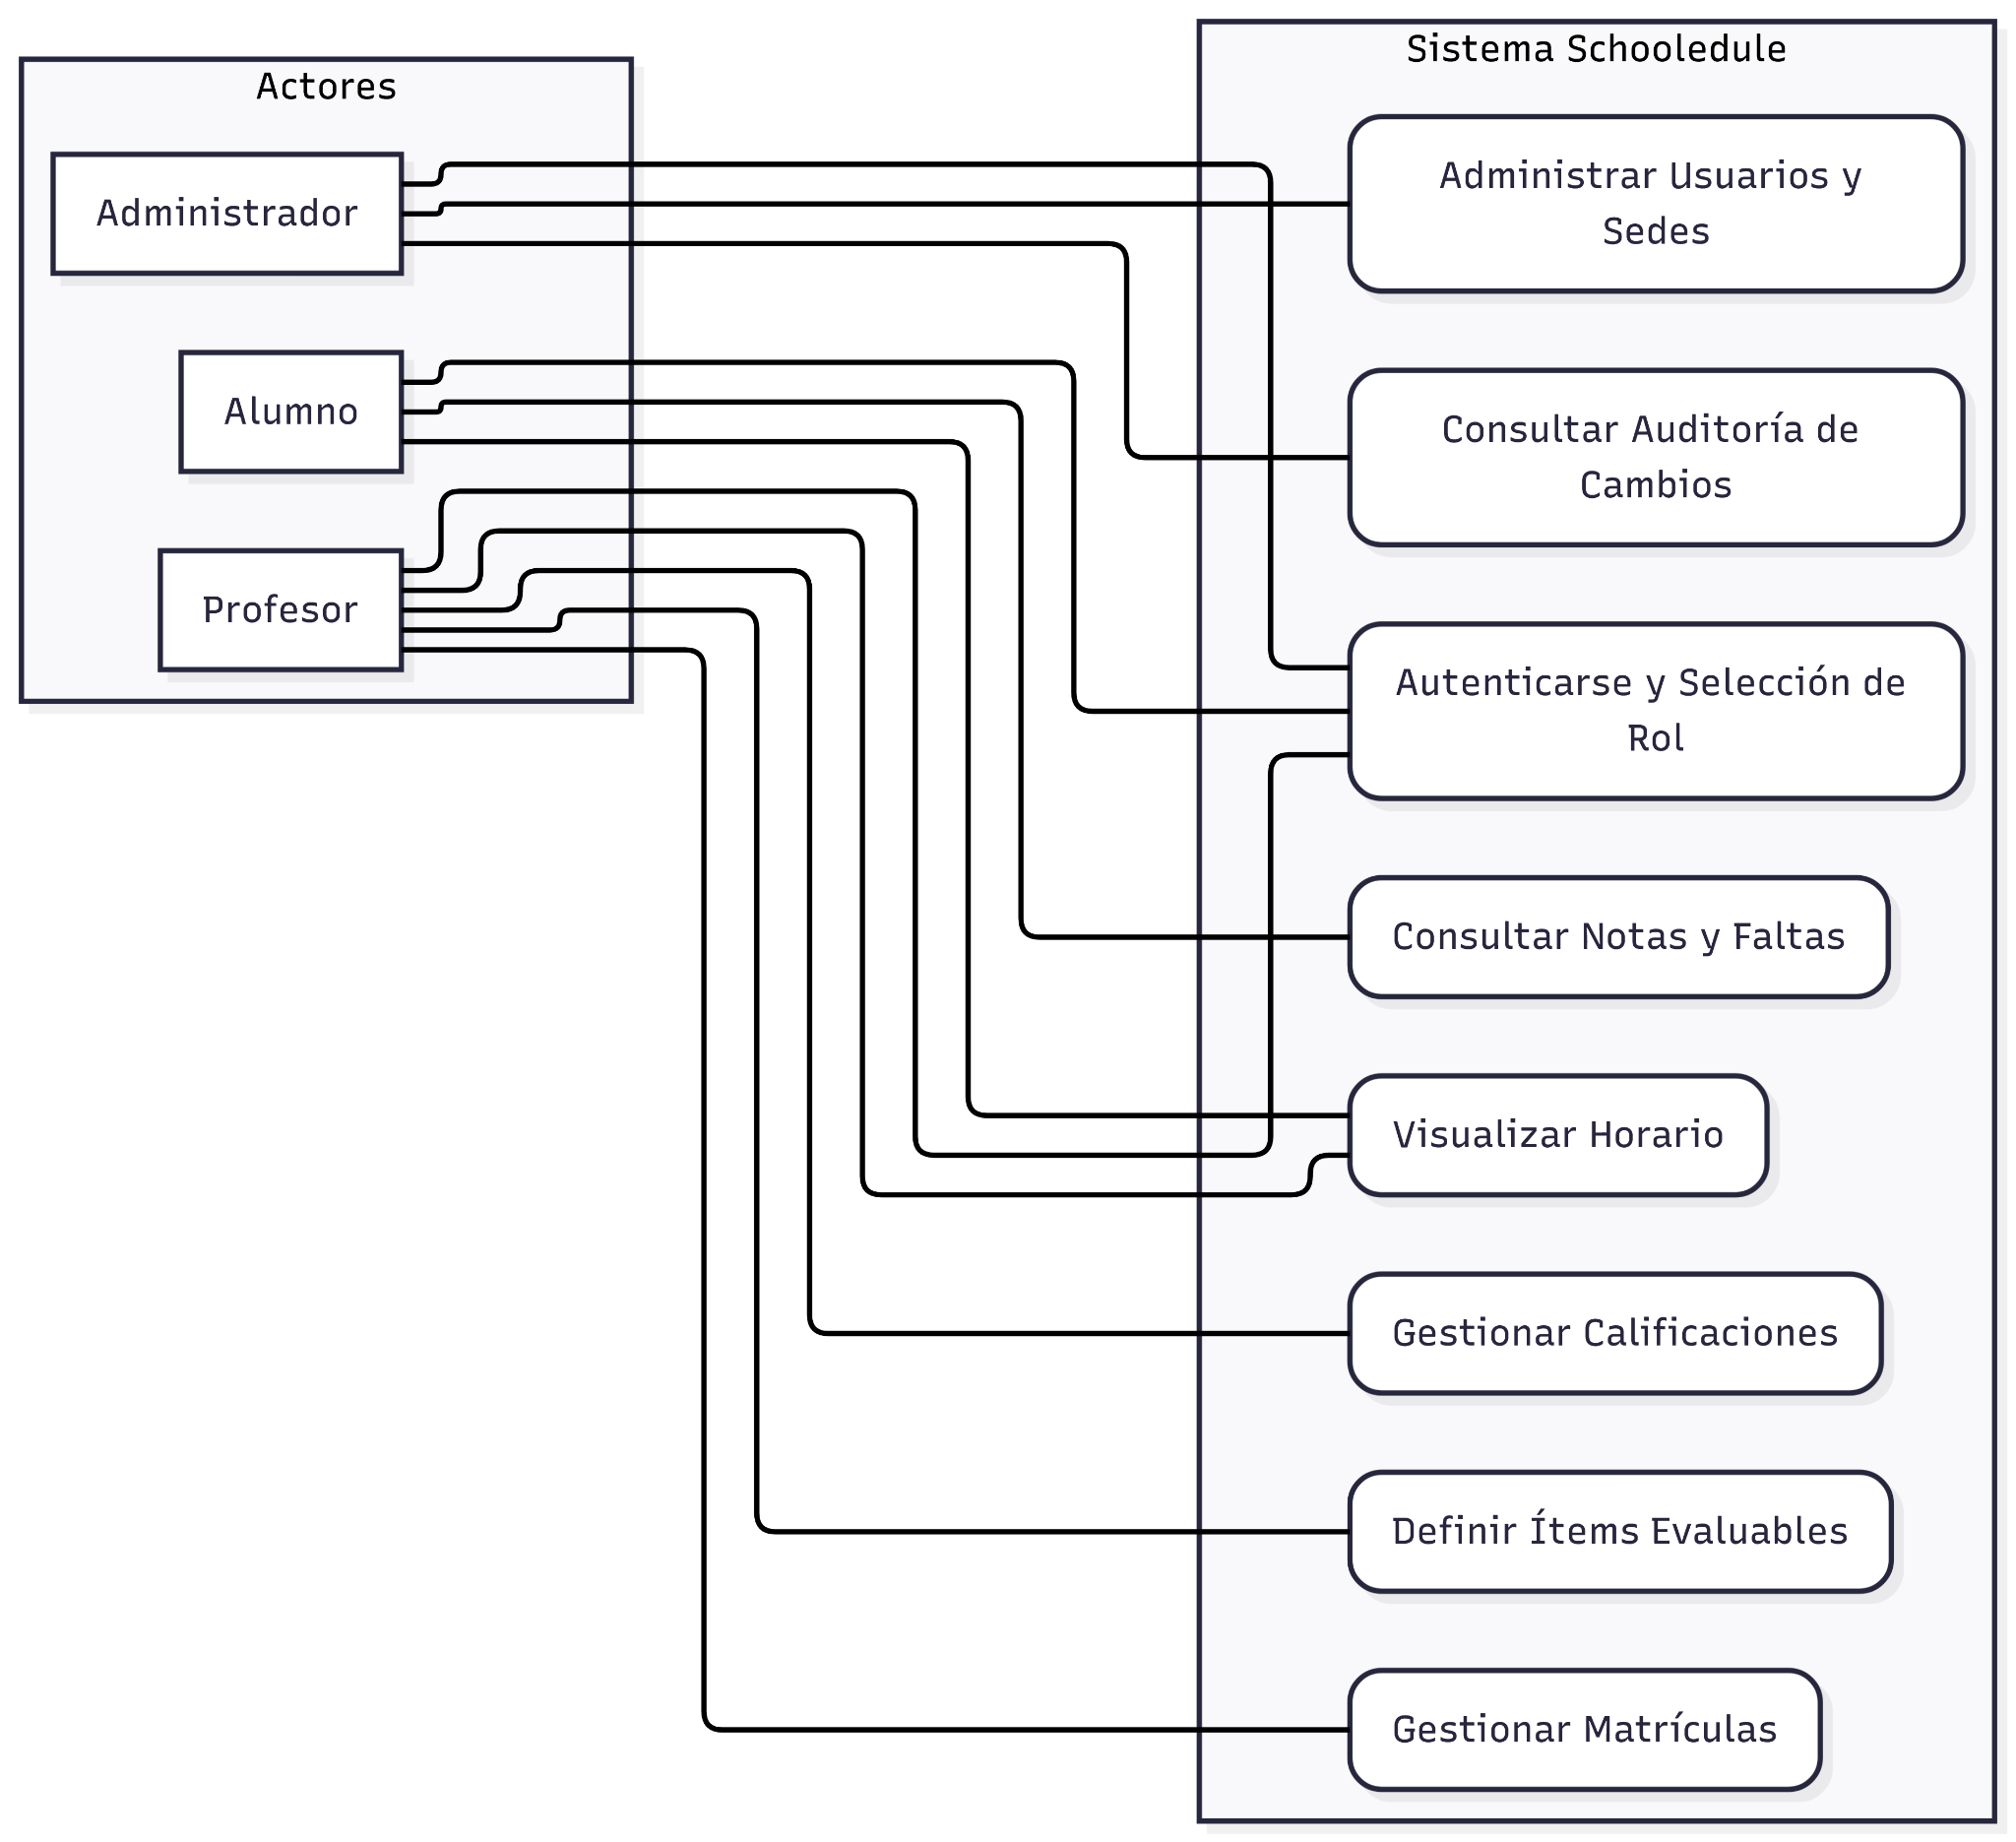
\includegraphics[width=0.9\textwidth]{figuras/image13.png}
    \caption{Diagrama de Clases del dominio Schooledule.}
    \label{fig:diagrama_clases}
\end{figure}

\section{Arquitectura de la Solución}
La solución se divide en tres capas principales:

\begin{enumerate}
    \item \textbf{Capa de Presentación}: Thymeleaf con Vanilla CSS y JavaScript para una interfaz limpia y eficiente.
    \item \textbf{Capa de Lógica de Negocio}: Spring Boot 3.3.5 orquestando todas las reglas académicas y validaciones RBAC.
    \item \textbf{Capa de Datos}: Persistencia en PostgreSQL con un sistema de auditoría forense inmutable.
\end{enumerate}

\begin{figure}[H]
    \centering
    
\includegraphics[width=1.0\textwidth]{figuras/image19.png}
    \caption{Diagrama Entidad-Relación (E/R) de la base de datos.}
    \label{fig:erd}
\end{figure}
